
\documentclass{subfiles}

\begin{document}
	

	
\par This research aims to ease the way of handling full-waveform (FW) LiDAR  data for remote forest surveys. The primary output of this thesis is the open source software DASOS (=forest in Greek), which aims to break the barrier between understanding and using the FW LiDAR (for more information about DASOS please refer to Section \ref{DASOS}). New representations of the FW LiDAR are further proposed for handling the data. The contributions of DASOS and the new representations of the FW LiDAR are demonstrated in three applications: 

\begin{itemize}
	\item Visualisations and optimisations on managing real volumetric data:
	
	\item Alignment with hyperspectral images for generating tree coverage maps:
	
	\item Dead Tree detection for managing biodiversity in Australian native forests:
	

\end{itemize}

\begin{figure}
	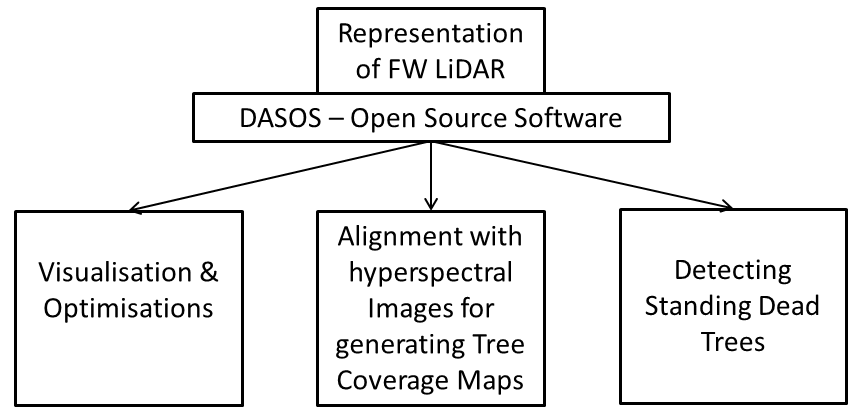
\includegraphics[width=\textwidth]{tex/Pipeline/Pipeline.png}
	\caption{The pipeline of the thesis}
\end{figure}



\end{document}


